\singlespacing

\mychapter{blue!45!black}{Discussion Générale}
	\sectionblue*{Résumé}
		\begin{center}
			\begin{tcolorbox}[colback=blue!5!white,colframe=blue!45!black,arc=0mm]
				\sffamily
				Après un bref récapitulatif des travaux effectués lors de cette thèse, nous traiterons dans cette conclusion l'importance que peuvent avoir les données initiales et la question biologique posée sur la performance des signatures, la taille des sous-réseaux et la significativité biologique des signatures.
				Nous analyserons ensuite les caractéristiques des signatures obtenues avec ITI en les comparant avec les signatures précédemment citées.
				Nous finirons cette discussion en exposant des perspectives sur l'évolution de l'algorithme et des analyses futures.
			\end{tcolorbox}
			\vspace{5ex}
			\mtcsetdepth{minitoc}{1}
			\minitoc
		\end{center}
		\newpage

\doublespacing

	\section{\textcolor{blue!45!black}{Rappels sur les travaux effectués}}
		\mylettrine{N}{ous avons dans cet ouvrage} exploré les caractéristiques biologiques des cancers et les spécificités du cancer du sein\index{cancer!cancer du sein}.
		Nous avons ensuite montré qu'une perturbation de l'expression et/ou la régulation des gènes pouvait être à l'origine du cancer.
		Nous avons rappelé l'intérêt des approches de médecines personnalisée et prédictive de classifier les tumeurs pour pouvoir les traiter de manière spécifique et proposer une thérapie adaptée.
		Après avoir exposé les limitations de l'approche transcriptomique à haut-débit pour étudier le cancer, nous avons détaillé notre méthode ITI, puis nous avons exposé les résultats d'une analyse non-supervisée et d'une analyse supervisée.

	\section{\textcolor{blue!45!black}{Importance des données initiales}}
		\mylettrine{L}{e jeu de données d'apprentissage} a une grande importance lors de l'établissement d'une signature prédictive, comme l'a montré \citeauthor{Michiels2005}.
		Ce phénomène est dû à la fois à la topologie des données et à la biologie du cancer (cf Section~\ref{def:limitations}).
		Notre approche intégrant simultanément plusieurs jeux de données transcriptome permet de moins dépendre des jeux de données initiaux.
		De plus, le fait d'homogénéiser les échantillons permet de minimiser la variation biologique dûe au cancer.
		Ainsi lors de la détection du sous-réseau, un gène n'ayant pas de variation d'expression dans un jeu de données peut être pris en compte pour la constitution d'un sous-réseaux, si son expression varie suivant les conditions cliniques dans un autre jeu de données (cf Section~\ref{sub:détection}).
		Avec un compendium de plusieurs jeux de données recouvrant 930 tumeurs, nous obtenons une performance de classification supérieure sur un jeu de données totalement indépendant comme nous l'avons montré dans l'exploration des résultats de notre analyse supervisée (cf Table~\ref{tab:Res2Classif}).
		Nous avons comparé les signatures réalisées avec ITI et les signatures issues de la littérature \citep{vandevijver2002,Wang2005,Sotiriou2006}.

	\section{\textcolor{blue!45!black}{Caractéristiques des signatures réalisées}}

		\subsection{\textcolor{blue!45!black}{Amélioration de la stabilité, robustesse et reproductibilité}}
			\mylettrine{P}{our comparer la pertinence} de nos sous-réseaux aux signatures déjà publiées, nous avons récupéré dans les articles originaux, les listes des sondes constituant la signature Mammaprint à 70 gènes \citep{vandevijver2002}, la signature statuts ER spécifique à 76 gènes \citep{Wang2005}, et la signature du \acs{GGI} \citep{Sotiriou2006}. Nous avons utilisé les annotations les plus récentes des sondes, enlevé les doublons, et n'avons pas considéré les EST. Les annotations des sondes étant constamment mises à jour, il peut y avoir une variation sur le nombre de gènes, c'est pourquoi nous trouvons un seul gène commun entre les signatures \citet{vandevijver2002} et \citet{Wang2005} alors que \citet{Chuang2007} en trouvaient 3. C'est également la raison pour laquelle la signature GGI \citep{Sotiriou2006} que nous avons réalisé contient 108 gènes (et non 97 comme précisé dans la littérature).
			La Figure~\ref{fig:Venn} compare les différentes signatures et notamment les gènes en communs.
			\begin{figure}
				\begin{center}
					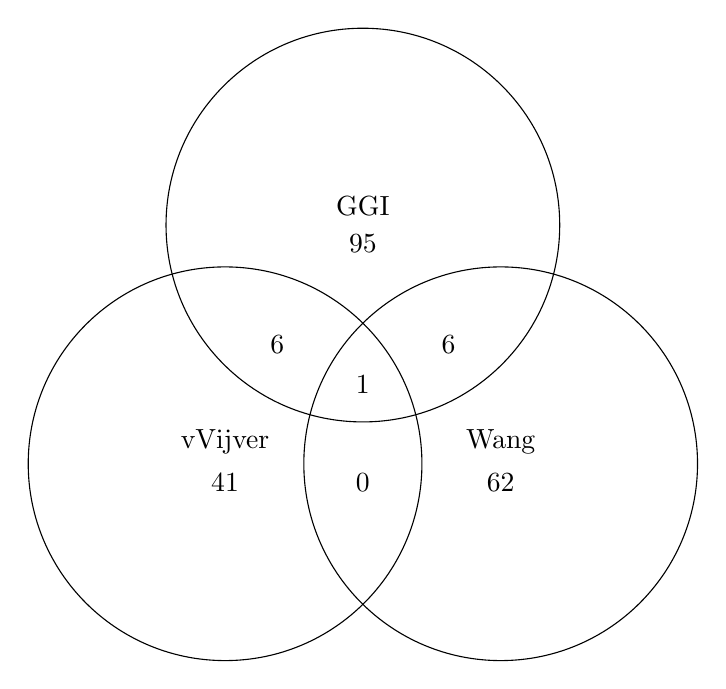
\begin{tikzpicture}
						\tikzset{venn circle/.style={draw,circle,minimum width=5cm}}
						\node [venn circle] (A) at (0,0)								{};
							\node [above]		at (A) 									{vVijver};
							\node [below]		at (A) 									{41};
						\node [venn circle] (B) at (60:3.5cm)							{};
							\node [above]		at (B) 									{GGI};
							\node [below]		at (B) 									{95};
						\node [venn circle] (C) at (0:3.5cm)							{};
							\node [above]		at (C) 									{Wang};
							\node [below]		at (C) 									{62};
							\node [left]		at (barycentric cs:A=1/2,B=1/2)			{6};
							\node [below]		at (barycentric cs:A=1/2,C=1/2)			{0};
							\node [right]		at (barycentric cs:B=1/2,C=1/2)			{6};
						\node					at (barycentric cs:A=1/3,B=1/3,C=1/3)	{1};
					\end{tikzpicture}
				\end{center}
				\caption{Diagramme de Venn comptabilisant les gènes communs entre les différentes signatures classiques.}\label{fig:Venn}
			\end{figure}

			Il apparaît que très peu de gènes sont communs entre ces signatures (moins de 5\% de la totalité des gènes des signatures deux à deux).
			À titre de comparaison, nous avons croisé les deux signatures ITI obtenues sur les échantillons ER+ et ER- avec nos deux études de notre analyse supervisée.
			Un total de 937 gènes sont communs entre nos deux signatures pour les échantillons ER-, et 46 gènes sont communs pour les signatures réalisées sur les échantillons ER+.
			Cela représente un recouvrement de respectivement 32.8\% (ER-) et 11.5\%(ER+).
			Ces valeurs relativement basses reflètent les biais dus aux jeux de données et aux plateformes de puces à ADN.
			Cependant, ce recouvrement est largement supérieur aux quelques gènes communs entre les autres signatures.
			Il pourrait être probablement augmenté en utilisant un ensemble de jeux de données d'entraînement plus large.

		\subsection{\textcolor{blue!45!black}{Significativité biologique relevante}}
			\mylettrine{R}{eprenant les trois signatures établies} dans la littérature (la signature Mammaprint à 70 gènes \citep{vandevijver2002}, la signature statuts ER spécifique à 76 gènes \citep{Wang2005}, et la signature du \acs{GGI} \citep{Sotiriou2006}), \citeauthor{HaibeKains2008} supposent que les pronostics sur le devenir des patients sont basés sur la représentation de processus biologiques qui se recouvrent largement.
			\citeauthor{Thomassen2007} ont comparé 9 signatures pronostiques, et ont trouvé que le cycle cellulaire et la prolifération cellulaire étaient les termes \acs{GO} les plus représentés.
			\citeauthor{Yu2007} ont conduit des analyses sur les différentes voies de régulation de 5 signatures prognostiques publiées avaient un grand nombre de voies en commun, comme le cycle cellulaire, la régulation du cycle cellaire, la mitose, l'apoptose, etc \dots
			\citeauthor{HaibeKains2008} ont étudié dans une méta-analyse à grande échelle des données publiques d'expression des gènes et ont trouvé que la prolifération était une force directrice commune d'un grand nombre de signatures pronostiques.
			Nous retrouvons dans nos analyses ces processus biologiques impliqués dans le cancer et la métastase, mais également d'autres processus, comme le contrôle des dommages à l'ADN et le système immunitaire qui sont également important.

		\subsection{\textcolor{blue!45!black}{Taille des sous-réseaux}}
			\mylettrine{L}{a question biologique} posée a son importance.
			Dans le cadre d'un cancer très hétérogène comme le cancer du sein, un nombre de gènes important est nécessaire pour réaliser une classifieur sur une question complexe comme la rechute métastatique.
			Si la question posée est la différentiation entre deux types de cancer où beaucoup de gènes sont différentiellement exprimés, comme pour la leucémie myéloïde aiguë et la leucémie lymphoblastique aiguë, peu de gènes peuvent suffire pour différencier les deux conditions cliniques \citet{Dobbin2008}.
			L'homogénéité des données a également son rôle dans la taille finale des sous-réseaux, comme nous l'avons vu précédemment.

	\section{\textcolor{blue!45!black}{Création d'une base de donnés de sous-réseaux}}
			\mylettrine{L}{a création d'une ressource} bioinformatique permettant l'exploration des sous-réseaux.
			Cette ressource, a été mise en place, accessible par Internet, contient pour chacune de nos analyses les sous-réseaux détectés statistiquement significatifs.
			Pour chacun des sous-réseaux, un enrichissement en termes \acs{GO} est calculé, par jeux de données d'expression, en se basant sur l'apport des gènes du sous-réseaux par rapport à l'ensemble des gènes présents sur la plateforme de puce à \acs{DNA} utilisée pour constituer le jeu de données.
			Cette ressource permet de relier l'interactome à la biologie de la maladie étudiée, ici dans le cadre du cancer du sein.
			Les sous-réseaux stockés étant discriminatifs pour la rechute métastatique dans le cancer du sein, leur exploration, facilitée par des analyses en enrichissement en termes \acs{GO} permet la découverte de gènes d'intérêts, non-liés précédemment au cancer du sein.
			Ces gènes d'intérêts peuvent être des cibles thérapeutiques potentielles, des \acsp{TSG} ou des oncogènes putatifs, ainsi que des gènes directeurs potentiels.
			
	\section{\textcolor{blue!45!black}{Perspectives}}
		\subsection{\textcolor{blue!45!black}{Améliorations de l'algorithme}}
			\mylettrine{L}{ors de cette thèse} nous avons pensé améliorer l'algorithme de détection de sous-réseaux, qui, en partant d'un gène graine, vérifie successivement et récursivement chacun des gènes voisins lors de la décision d'ajout d'un gène ou non sur le sous-réseau.
			L'algorithme explore donc l'interactome de façon linéaire, et l'ajout d'un gène voisin peut alors influencer la décision d'ajout d'un gène à la même distance de la graine.
			Nous pouvons modifier cet étape pour réaliser une exploration circulaire de l'espace interactome.
			Toujours en partant d'un gène graine, l'algorithme vérifierait donc simultanément tous les gènes voisins de même rang, et ajouterai ou non ceux qui améliorent le score du sous-réseaux.
			L'ajout des gènes de même rang se faisant de façon simultanée, il ne pourrait donc plus y avoir d'influence à l'ajout d'un gène sur l'ajout d'un autre gène de même rang.

		\subsection{\textcolor{blue!45!black}{Intégration d'autres types de données}}
			\mylettrine{N}{ous avons réalisé} des analyses pour inclure des informations de variabilité du nombre de copies des gènes dans le chapitre "\emph{CNV-Interactome-Transcriptome Integration to detect driver genes in cancerology}" \citep{Garcia2013b}.
			Nous allons prochainement explorer la biologie particulière de certains sous-types du cancer du sein, comme les Claudin-low.
			Des travaux seront également réalisés pour inclure des données épigénétiques (méthylation de l'ADN), ainsi que des informations sur les \acsp{miRNA}.

		\subsection{\textcolor{blue!45!black}{Étude de l'importance de la nature de l'interaction}}
			\mylettrine{D}{ans le but d'étudier} l'impact de la nature des différents types d'interactions sur la nature des sous-réseaux et la performance des signatures ainsi obtenues, nous allons réaliser des analyses en variant les jeux de données d'interactions utilisés.
			Le lien étroit entre interactions protéines-protéines et le niveau d’expression des gènes, déjà évoqué lors de l'explication de la validation statistique (cf Section~\ref{sec:Validation}) laisse supposer que l'utilisation d'un interactome plus bruité (\emph{ie} un interactome contenant en plus des informations fausses sur les interactions protéines-protéines) aura peu d'impact.
			En effet l'utilisation d'un interactome aléatoire ne permet la création que d'un faible nombre de sous-réseaux.
			Nous supposons de plus qu'un interactome plus complet aura un impact positif sur la détection des sous-réseaux et sur la performance des signatures.

	\section{\textcolor{blue!45!black}{Conclusion}}
		\mylettrine{A}{près un rappel} des travaux réalisés, nous avons expliqué l'impact des données initiales et de la complexité de la question biologique posée sur les caractéristiques des signatures découvertes avec ITI.
		Nous avons également comparé les signatures découvertes avec ITI avec les signatures déjà publiées \citep{vandevijver2002,Wang2005, Sotiriou2006}.
		Nous allons maintenant aborder dans la dernière partie notre conclusion générale.